\clearpage
\section{M-QAM Transmission System}

\begin{tcolorbox}	
	\begin{tabular}{p{2.75cm} p{0.2cm} p{10.5cm}} 	
		\textbf{Student Name}  &:& Ana Luisa Carvalho (2017/04/01 - 2017/12/31) \\
		\textbf{Goal}          &:& M-QAM system implementation with BER measurement and comparison with theoritical values.\\
		\textbf{Directory} &:& sdf/m\_qam\_system
	\end{tabular}
\end{tcolorbox}

The goal of this project is to simulate a Quadrature Amplitude Modulation transmission system with M points in the constellation diagram (M-QAM) and to perform a Bit Error Rate (BER) measurement that can be compared with theoretical values. 

M-QAM systems can encode $\log_2 M$ bits per symbol which means they can transmit higher data rates keeping the same bandwidth when compared, for example, to PSK systems. However, because the states are closer together, these systems are more susceptible to noise.

The Bit Error Rate (BER) is a measurement of how a bit stream is altered by a transmission system due to noise (among other factors). To study this effect we introduced Additive White Gaussian Noise (AWGN) to model thermal noise at the receiver. 

For $M=4$ the M-QAM system reduces to a Quadrature Phase Shift Keying system (QPSK) system that uses four equispaced points in the constellation diagram (see figure \ref{fig:const}). 

\begin{figure}[h]
	\centering
	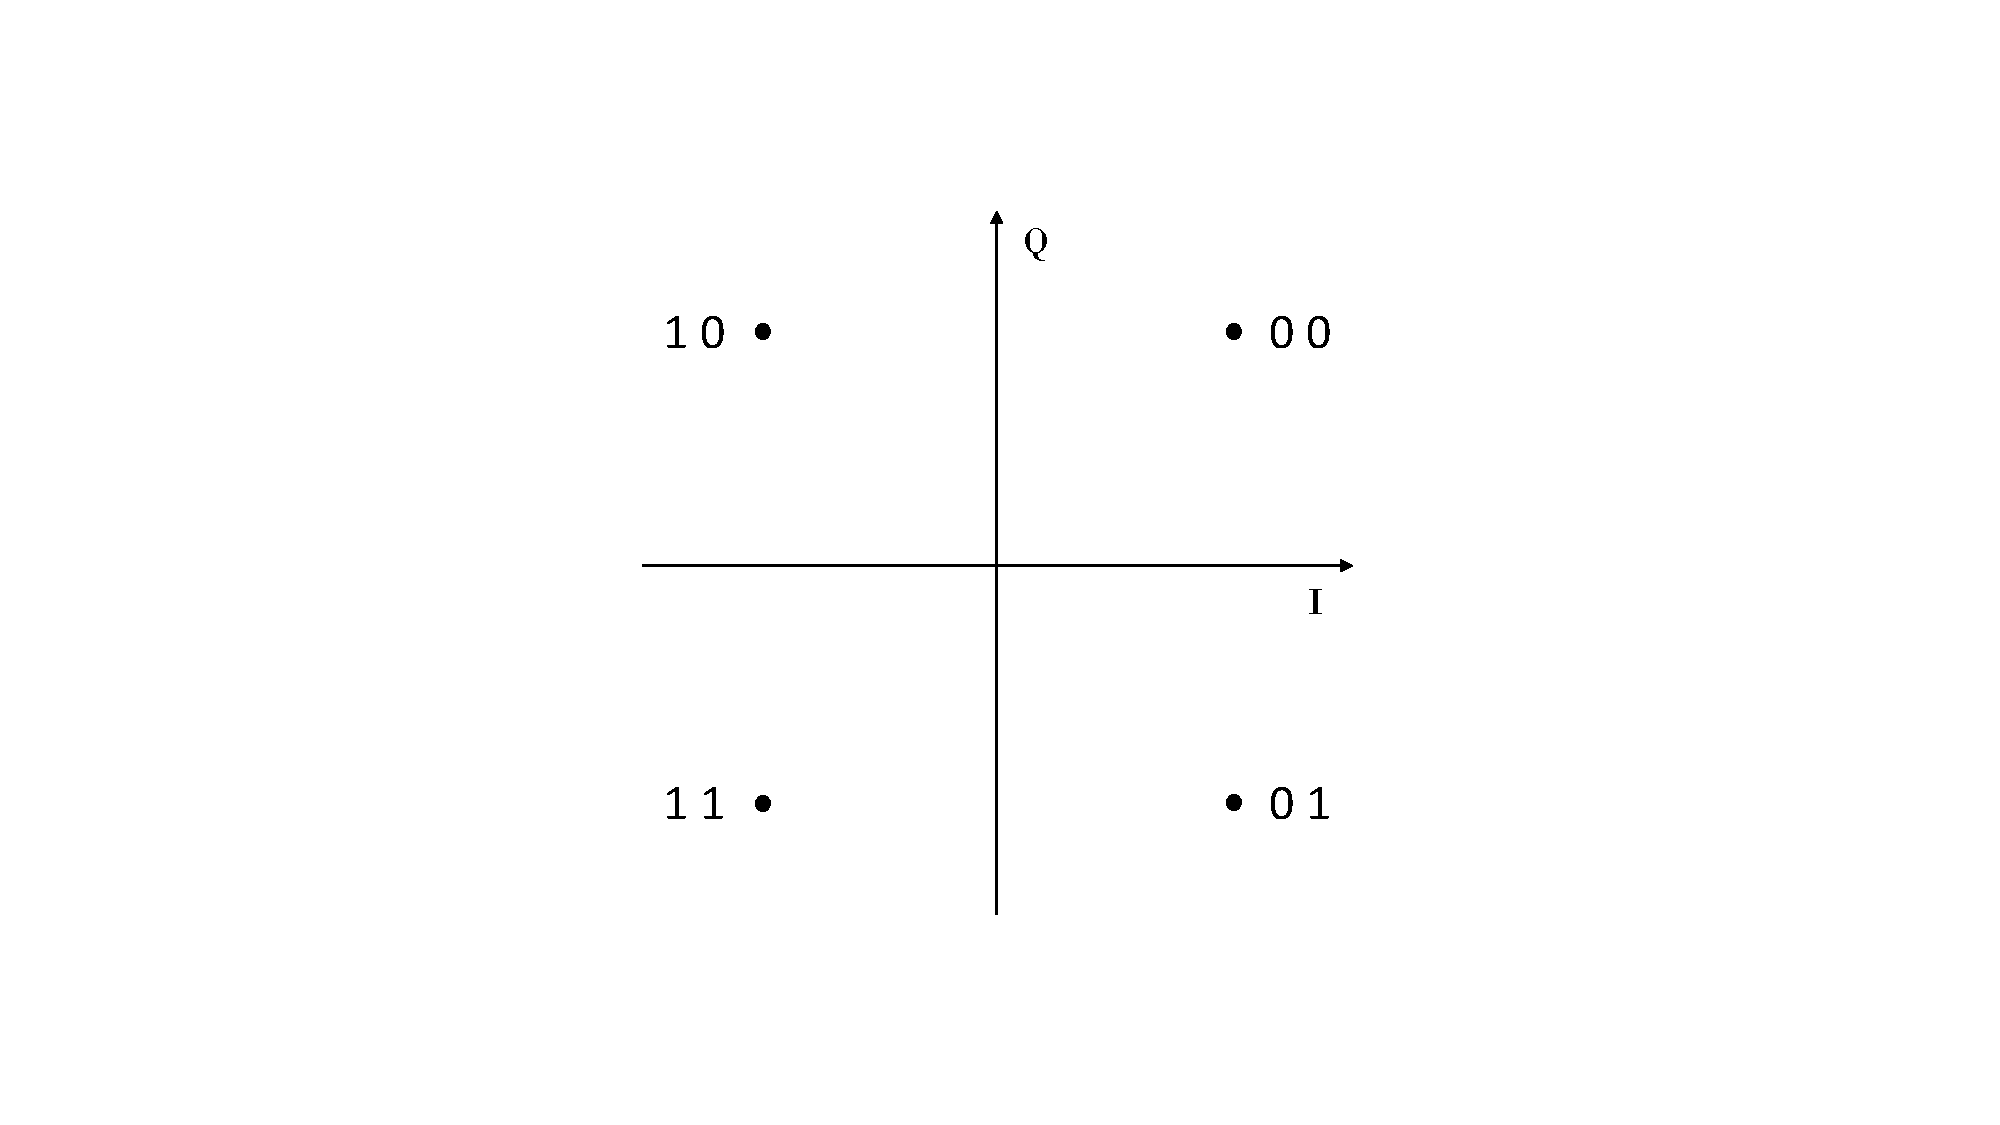
\includegraphics[clip, trim=3cm 3cm 3cm 3cm, width=\textwidth]{./sdf/m_qam_system/figures/MQAM_constellation.pdf}
	\caption{4-QAM constellation points.}
	\label{fig:const}
\end{figure}

%M can take several values: $2, 4, 16, 32, ...$. The first two correspond to BPSK and QPSK modulation, respectively.

\subsection{Theoretical Analysis }

M-QAM is a modulation scheme that takes advantage of two carriers (usually sinusoidal waves) with a phase difference of $\frac{\pi}{2}$. The resultant output consists of a signal with both amplitude and phase variations. The two carriers, refered to as I (In-phase) and Q (Quadrature), can be represented as 

\begin{align}
	I=A\cos(\phi) \\
	Q=A\sin(\phi)
\end{align}
which means that any sinusoidal wave can be decomposed in its I and Q components:

\begin{align}
	A\cos(\omega~t+\phi)&=A\left(\cos(\omega~t)\cos(\phi)-\sin(\omega~t)\sin(\phi)\right) \\
	&=I\cos(\omega~t)-Q\sin(\omega~t),
\end{align} 
where we have used the expression for the cossine of a sum and the definitions of I and Q.

%When demodulating a signal it is necessary to associate the received signal to the corresponding signal. The existence of noise in the channel means that we can only compute the probability that a given signal corresponds to a certain carrier and that's why we need to define the BER. Using
%
%\begin{equation}
%P_i f(s|c_i)>P_j f(s|c_j), \qquad i\neq j
%\end{equation}
%where $f(s|c_i)$ stands for the probability of detecting the signal $s$ given that $c_i$ was emmited. This inequallity can be rewritten in the following way
%
%\begin{equation}
%P(c_i|s)>P(c_j|s)
%\end{equation}
%where $P(c_i|s)$ and $P(c_j|s)$ are called \textit{a posteriori} probabilities and represent the probability that $c_i$ or $c_j$ were transmitted given that $s$ was received. In terms of the systems this simply means that we should select the signal most likely to have been transmitted.
%
%In the case of additive white gaussian noise the $f$ function is simply given by
%
%\begin{equation}
%f(s|c_i)=\frac{e^{-x^2/n_0}}{(\pi n_0)^{N/2}}
%\end{equation}
%where $x$ is the Euclidean distance in the I-Q plane between the signal received and carrier i and $N$ is the number of noise samples.
%
%When using 4-QAM modulation all points are at an equal distance from the origin (in the I-Q plane) so they all have the same energy given by
%
%\begin{equation}
%E=\frac{d^2}{2}
%\end{equation}
%where $d$ is the side of the square formed bye the constellation points.
%
%The probability that a given signal is identified correctly is given by
%
%\begin{equation}
%P_c=r^2
%\end{equation}
%where $n_0/2$ is the noise variance for AWGN and
%
%\begin{equation}
%r=\int_{-d/2}^{\infty}\frac{e^{-x^2/n_0}}{\sqrt{\pi n_0}} dx.
%\end{equation}
%
%The error probability, $P_e$, given by $1-P_c$ is given by
%
%\begin{equation}
%P_e=\erfc \sqrt{\frac{E}{2 n_0}}.
%\end{equation}

The probability of symbol error, $P_s$, in coherent M-PSK demodulation with AWGN is given by 

\begin{equation}
	P_s=2~Q\left(\sqrt{2~\log_2 M \left(\frac{E_b}{n_0}\right)\sin^2\frac{\pi}{M}}\right)
\end{equation}
where $E_b$ is the energy of one bit, $n_0$ is the noise power and the function $Q$ is defined as
\begin{equation}
	Q(x)=\frac{1}{2} erfc\left(\frac{x}{\sqrt{2}}\right).
	\label{eq:Ps}
\end{equation}

The probability of bit errors, $P_b$ is related to $P_s$ by
\begin{equation}
	P_b=\frac{1}{\log_2 M}P_s.
	\label{eq:Pb}
\end{equation} 

For QPSK we get, using $M=4$ in equations \ref{eq:Ps} and \ref{eq:Pb},
\begin{equation}
	P_b=\frac{1}{2} erfc\left(\sqrt{\frac{2~E_b}{n_0}}\right).
\end{equation}

This function is plotted in figure \ref{fig:QPSK_th_curve} for $n_0=10^{-6}$.

\begin{figure}[h]
		\centering
		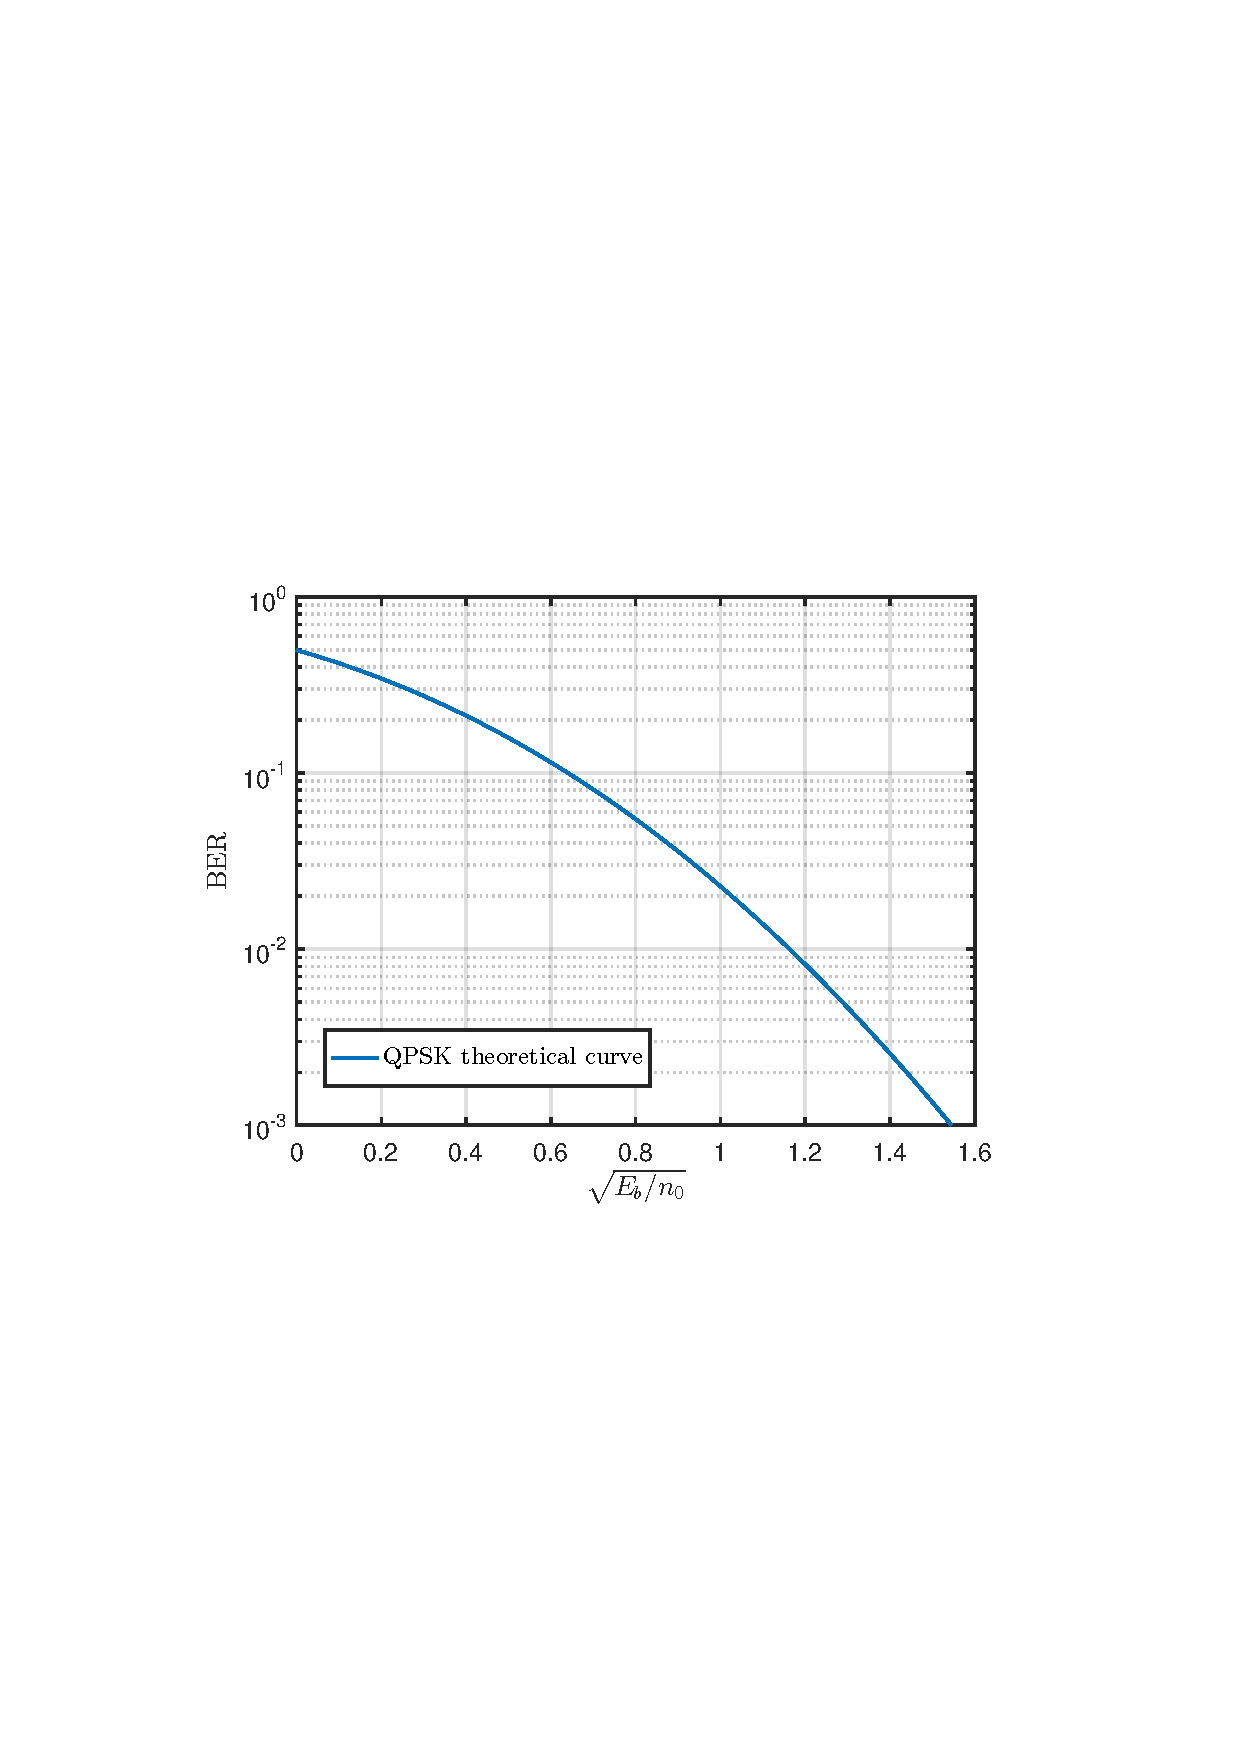
\includegraphics[clip, trim=0.5cm 9cm 0.5cm 9cm, width=\textwidth]{./sdf/m_qam_system/figures/BER_QPSK_theory_Eb_n0.pdf}
		\caption{QPSK theoretical BER values as a function of the output optical power in dBm.}
		\label{fig:QPSK_th_curve}
\end{figure}

\pagebreak
\subsection{Simulation Analysis}

The system to be simulated is composed of four blocks: a M-QAM transmitter, a M-QAM receiver, a sink and a block that performs a Bit Error Rate (BER) measurement. This system is a complex block of code that simulates the modulation, transmission and demodulation of an optical signal using M-QAM modulation. The schematic representation of the
system is presented in figure \ref{MQAM_system_block_diagram}. 

\begin{figure}[!b]
	\centering
	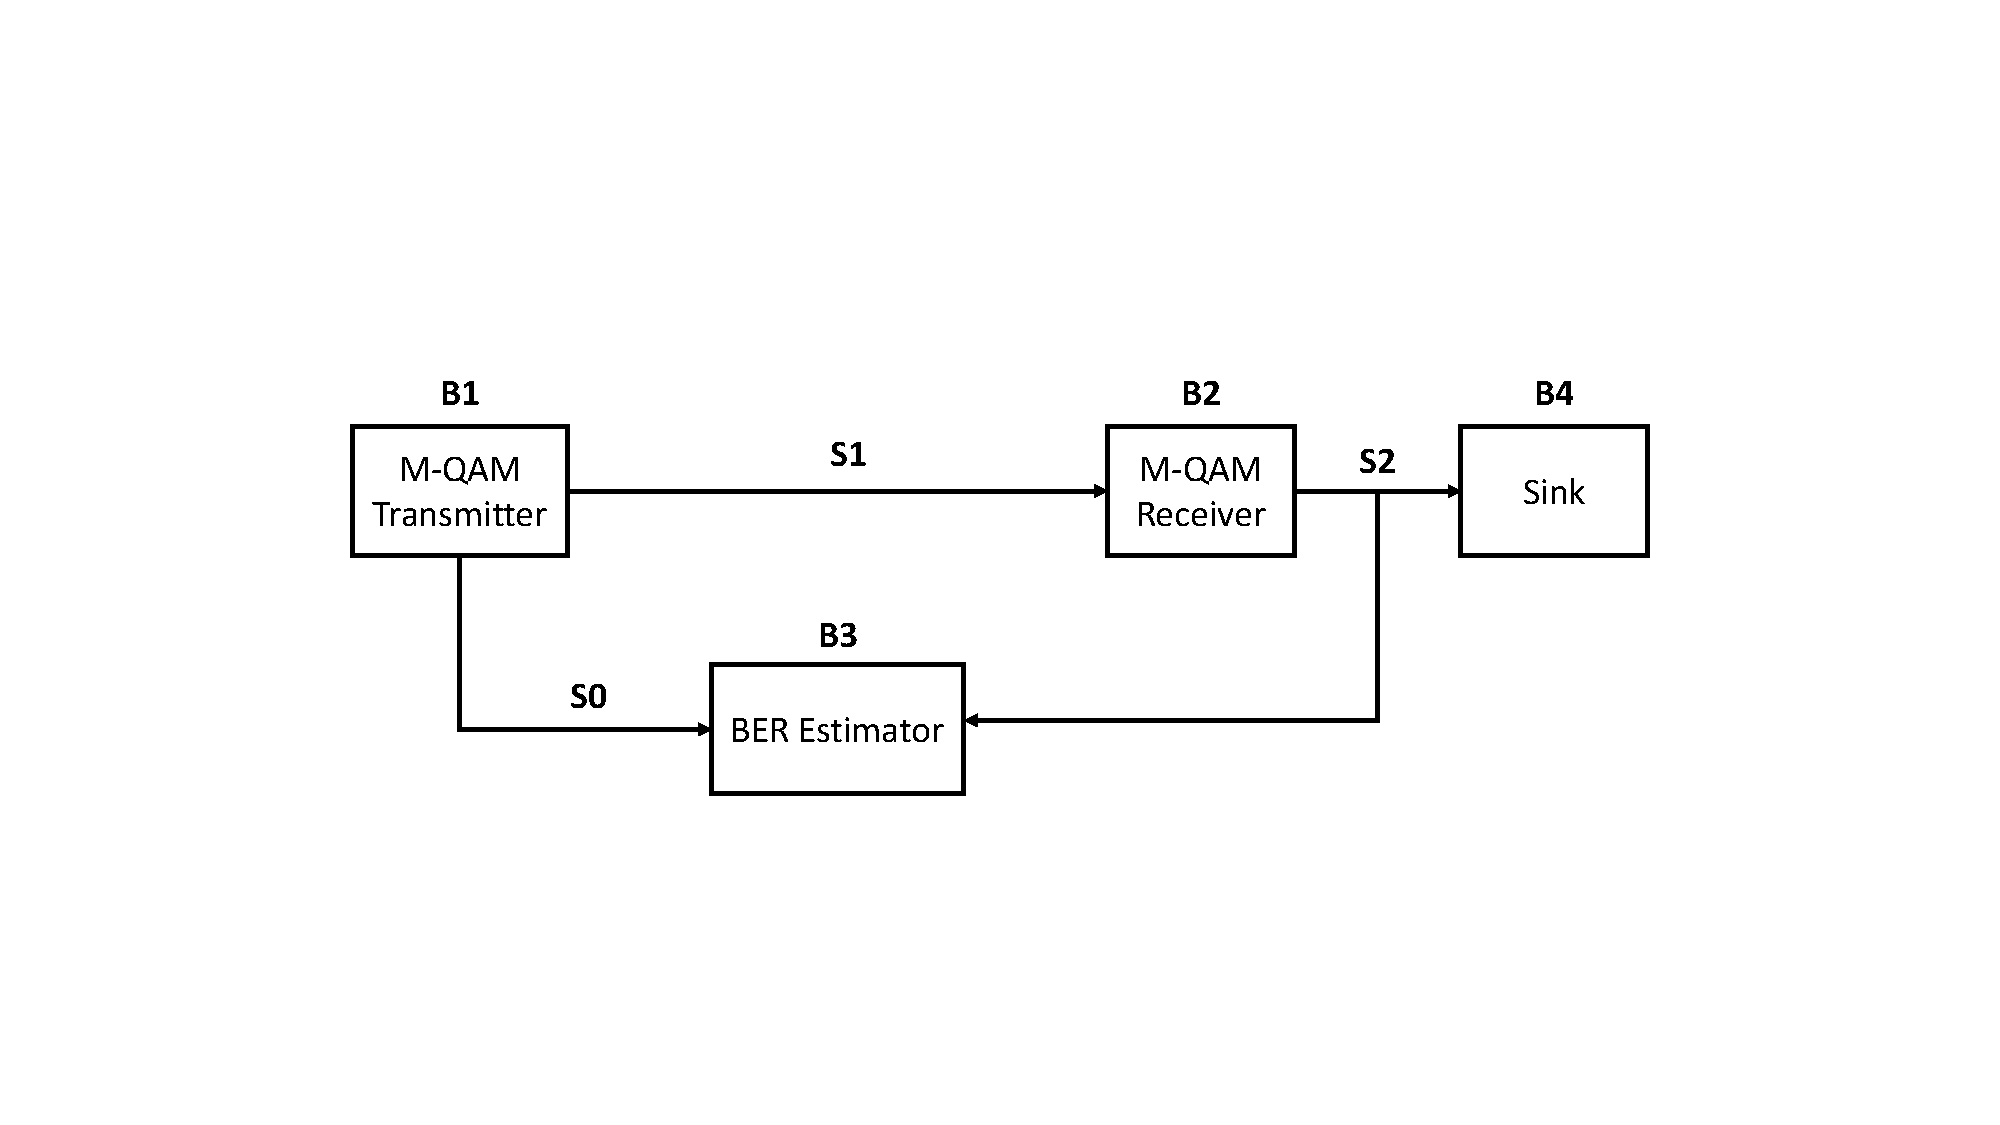
\includegraphics[trim={4cm 4cm 4cm 6cm},clip,width=\textwidth]{./sdf/m_qam_system/figures/MQAM_system_block_diagram.pdf}
	\caption{Schematic representation of the M-QAM system.}\label{MQAM_system_block_diagram}
\end{figure}

%The M-QAM transmission system is a complex block of code that simulates the modulation, transmission and demodulation of an optical signal using M-QAM modulation.

\paragraph{Current state:} The system currently being implement is a QPSK system (M=4).

\paragraph{Future work:} Extend this block to include other values of M.

\subsection*{Functional description}

A complete description of the M-QAM transmitter and M-QAM homodyne receiver blocks can be found in the \textit{Library} chapter of this document as well as a detailed description of the independent blocks that compose these blocks.

The M-QAM transmitter generates one or two optical signals by enconding a binary string using M-QAM modulation. It also outputs a binary signal that is used to perform the BER measurement.

The M-QAM homodyne receiver accepts one input optical signal and outputs
a binary signal. It performs the M-QAM demodulation of the input signal by combining the optical signal with a local oscillator.

The demodulated optical signal is compared to the one produced by the transmitter in order to estimate the Bit Error Rate (BER).

\subsection*{Input Parameters}

The system accepts several input parameters that can be defined by the user. These are described in table \ref{table:in_par}.

\begin{table}[h]
	\centering
	\caption{Input parameters}
	\begin{tabular}{|c|c|p{70mm}|ccp{70mm}}
		\cline{1-3}
		\textbf{Parameter} & \textbf{Type} & \textbf{Description} &    \\ \cline{1-3}
		%numberOfBitsGenerated & t\_integer & Determines the number of bits to be generated by the binary source  &    \\ \cline{1-3}
		%samplesPerSymbol & t\_integer & Number of samples per symbol &    \\ \cline{1-3}
		%prbsPatternLength & int & Determines the length of the pseudorandom sequence pattern (used only when the binary source is operated in \textit{PseudoRandom} mode) &    \\ \cline{1-3}
		%bitPeriod & t\_real & Temporal interval occupied by one bit &    \\ \cline{1-3}
		%rollOffFactor & t\_real & Parameter of the raised cosine filter &    \\ \cline{1-3}
		signalOutputPower\_dBm & t\_real & Determines the power of the output optical signal in dBm &  \\ \cline{1-3}
		numberOfBitsReceived & int &   Determines when the simulation should stop. If $-1$ then it only stops when there is no more bits to be sent&   \\ \cline{1-3}
		iqAmplitudeValues & vector<t\_iqValues> & Determines the constellation used to encode the signal in IQ space &    \\ \cline{1-3}
		%symbolPeriod & double & Given by bitPeriod/samplesPerSymbol &    \\ \cline{1-3}
		%localOscillatorPower\_dBm & t\_real & Power of the local oscillator &    \\ \cline{1-3}
		%responsivity & t\_real & Responsivity of the photodiodes (1 corresponds to having all optical power transformed into electrical current) &    \\ \cline{1-3}
		%amplification & t\_real & Amplification provided by the ideal amplifier &    \\ \cline{1-3}
		%noiseAmplitude & t\_real & Amplitude of the white noise &    \\ \cline{1-3}
		%samplesToSkip & t\_integer & Number of samples to be skipped by the \textit{sampler} block &    \\ \cline{1-3}
		%confidence & t\_real & Determines the confidence limits for the BER estimation &    \\ \cline{1-3}
		%midReportSize & t\_integer &  &    \\ \cline{1-3}
		%bufferLength & t\_integer & Corresponds to the number of samples that can be processed in each run of the system &    \\ \cline{1-3}
	\end{tabular}
	\label{table:in_par}
\end{table}

\subsection*{Required Files}

The required header and source files needed to run this system are summarized in table \ref{table:files}.

\begin{table}[]
	\centering
	\label{files_table}
	\caption{Main system files}
	\begin{tabular}{|c|c|p{35mm}|c|ccc}
		\cline{1-4}
		\textbf{Source file} & \textbf{Header file}  &  \textbf{System blocks} & \textbf{Status} & \\ \cline{1-4}
		m\_qam\_system\_sdf.cpp & --- & Main &\checkmark & \\ \cline{1-4}
		m\_qam\_transmitter.cpp & m\_qam\_transmitter.h & M-QAM Transmitter & \checkmark &  \\ \cline{1-4}
		m\_qam\_homodyne\_receiver.cpp & homodyne\_receiver.h & M-QAM Receiver & \checkmark &  \\ \cline{1-4}
		sink.cpp & sink.h & Sink & \checkmark & \\ \cline{1-4}
		bit\_error\_rate.cpp & bit\_error\_rate.h & BER Estimator & \checkmark &\\ \cline{1-4}
		add.cpp & add.h & M-QAM transmitter & \checkmark & \\ \cline{1-4}
		binary\_source.cpp & binary\_source.h & M-QAM Transmitter & \checkmark & \\ \cline{1-4}
		discrete\_to\_continuous\_time.cpp & discrete\_to\_continuous\_time.h & M-QAM Transmitter & \checkmark & \\ \cline{1-4}
		ideal\_amplifier.cpp & ideal\_amplifier.h & M-QAM Receiver & \checkmark & \\ \cline{1-4}
		iq\_modulator.cpp & iq\_modulator.h & M-QAM Transmitter & \checkmark & \\ \cline{1-4}
		local\_oscillator.cpp & local\_oscillator.h & M-QAM Receiver & \checkmark & \\ \cline{1-4}
		m\_qam\_mapper.cpp & m\_qam\_mapper.h & M-QAM Transmitter & \checkmark & \\ \cline{1-4}
		netxpto.cpp & netxpto.h & All & \checkmark & \\ \cline{1-4}
		optical\_hybrid.cpp & optical\_hybrid.h & M-QAM Receiver & \checkmark & \\ \cline{1-4}
		photodiode\_old.cpp & photodiode\_old.h & M-QAM Receiver & \checkmark & \\ \cline{1-4}
		pulse\_shaper.cpp & pulse\_shaper.h & M-QAM Transmitter \newline M-QAM receiver & \checkmark & \\ \cline{1-4}
		sampler\_20171119.cpp & sampler\_20171119.h & M-QAM Receiver & \checkmark & \\ \cline{1-4}
		sink.cpp & sink.h & Sink & \checkmark & \\ \cline{1-4}
		super\_block\_interface.cpp & super\_block\_interface.h & ? & \checkmark & \\ \cline{1-4}
		white\_noise.cpp & white\_noise.h & M-QAM Receiver & \checkmark & \\ \cline{1-4}
	\end{tabular}
	\label{table:files}
\end{table}

%\begin{table}
% 	\centering
% 	\caption{Required files}
% 	\begin{tabular}{|c|c|p{40mm}|c|ccp{40mm}c}
% 		\cline{1-4}
% 		\textbf{Header file} & \textbf{Source file} & \textbf{Description} &  \textbf{Status} & \\ \cline{1-4}
% 		add.h & add.cpp & Adds two signals.  & \checkmark &   \\ \cline{1-4}
% 		binary\_source.h & binary\_source.cpp & Produces a binary sequence. & \checkmark & \\ \cline{1-4}
% 		bit\_error\_rate.h & bit\_error\_rate.cpp & Computes the BER and writes it to a text file. & \checkmark & \\ \cline{1-4}
% 		discrete\_to\_continuous\_time.h & discrete\_to\_continuous\_time.cpp & Converts a signal from discrete in time to continuous in time. & \checkmark & \\ \cline{1-4}
% 		homodyne\_receiver.h & m\_qam\_homodyne\_receiver.cpp & & \\ \cline{1-4}
% 		ideal\_amplifier.h & ideal\_amplifier.cpp & Amplifies the signal. & \checkmark & \\ \cline{1-4}
% 		iq\_modulator.h & iq\_modulator.cpp & Divides the signal in its quadrature and in phase components & \checkmark &\\ \cline{1-4}
% 		local\_oscillator.h & local\_oscillator.cpp & & & \checkmark &\\ \cline{1-4}
% 		m\_qam\_mapper.h & m\_qam\_mapper.cpp & Maps the signal using the defined constellation & \checkmark & \\ \cline{1-4}
% 		m\_qam\_transmitter.h & m\_qam\_transmitter.cpp & & \checkmark & \\ \cline{1-4}
% 		netxpto.h & netxpto.cpp & General class that contains definition from signals and buffers. & \checkmark &\\ \cline{1-4}
% 		optical\_hybrid.h & optical\_hybrid.cpp & Implements an optical hybrid. & \checkmark & \\ \cline{1-4}
% 		photodiode\_old.h & photodiode\_old.cpp & Pair of photodiodes and current subtraction. & \checkmark & \\ \cline{1-4}
% 		pulse\_shaper.h & pulse\_shaper.cpp & Electrical filter. & \checkmark &\\ \cline{1-4}
% 		sampler\_20171119.h & sampler\_20171119.cpp & Samples the signal. & \checkmark &\\ \cline{1-4}
% 		sink.h & sink.cpp & Deletes signal. & \checkmark & \\ \cline{1-4}
% 		super\_block\_interface.h & super\_block\_interface.cpp & & \checkmark &\\ \cline{1-4}
% 		white\_noise.h & white\_noise.cpp & Generates white gaussian noise. & \checkmark &\\ \cline{1-4}  
% 	\end{tabular}
% 	\label{table:files}
%\end{table}

\pagebreak
\subsection*{Simulation results}

The parameters used to produce the results presented in this section are summarized in table \ref{table:par}.

\begin{table}[]
	\centering
	\caption{Values of the simulation parameters}
	\begin{tabular}{|c|c|cc}
		\cline{1-2}
		\textbf{Parameter} & \textbf{Value} & \\ \cline{1-2}
		numberOfBitsGenerated & $4000$ & \\ \cline{1-2}
		samplesPerSymbol & $16$ & \\ \cline{1-2}
		bitPeriod & $20$~ps & \\ \cline{1-2}
		rollOfFactor & $0.9$ & \\ \cline{1-2}
		prbsPatternLength & $7$ & \\ \cline{1-2}
		symbolPeriod & $1.25$~ps & \\ \cline{1-2}
		localOscillatorPower\_dBm & $0$ & \\ \cline{1-2}
		localOscillatorPhase & $0$ & \\ \cline{1-2}
		responsivity & $1$ & \\ \cline{1-2}
		amplification & $10^3$ & \\ \cline{1-2}
		noiseAmplitude & $10^{-6}$ & \\ \cline{1-2}
		samplesToSkip & $256$ & \\ \cline{1-2}
		confidence & $0.95$ & \\ \cline{1-2}
		midReportSize & $0$ & \\ \cline{1-2}
		bufferLength & $512$ & \\ \cline{1-2}
	\end{tabular}
	\label{table:par}
\end{table}

We show the eye diagrams for the signals HMD14 and HMD15 (see figure \ref{fig:MQAM_receiver}) for $\sqrt{\frac{E_b}{n_0}}=10^{-8},1,10^6$. These correspond to figures \ref{fig:eye_diagram_140}, \ref{fig:eye_diagram_60}, \ref{fig:eye_diagram_0}, respectively. We also show, in figure \ref{fig:ber_pseudorandom_sim}, the plot of the BER as a function of $\sqrt{\frac{E_b}{n_0}}$.

\begin{figure}[]
	\centering
	\includegraphics[width=1.1\textwidth]{./lib/homodyne_receiver/figures/MQAM_receiver_block_diagram.png}
	\caption{M-QAM receiver schematic representation}
	\label{fig:MQAM_receiver}
\end{figure}

\begin{figure}
	\centering
	\begin{subfigure}{.5\textwidth}
		\centering
		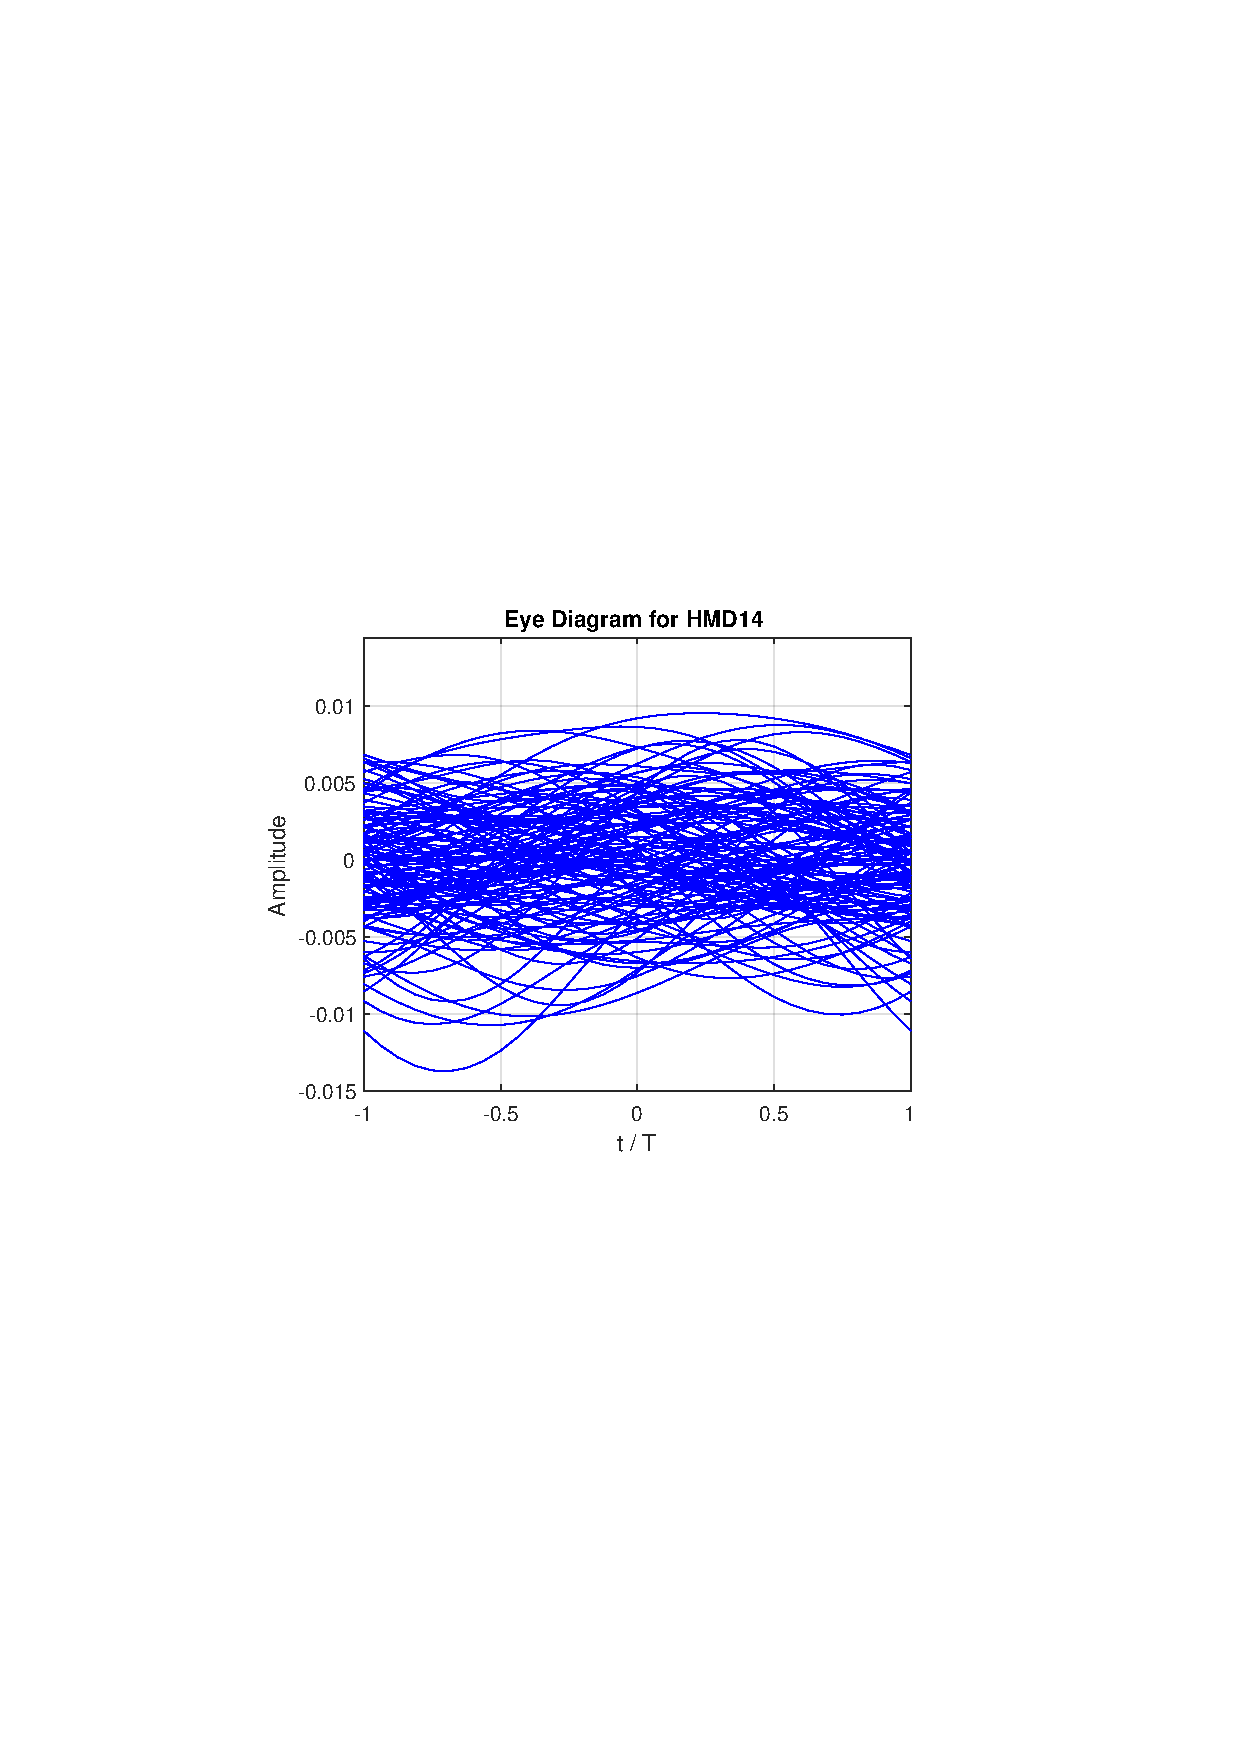
\includegraphics[clip, trim=5cm 10cm 5cm 10cm, width=\textwidth]{./sdf/m_qam_system/figures/HMD14_eye_diagram_140.pdf}
	\end{subfigure}%
	\begin{subfigure}{.5\textwidth}
		\centering
		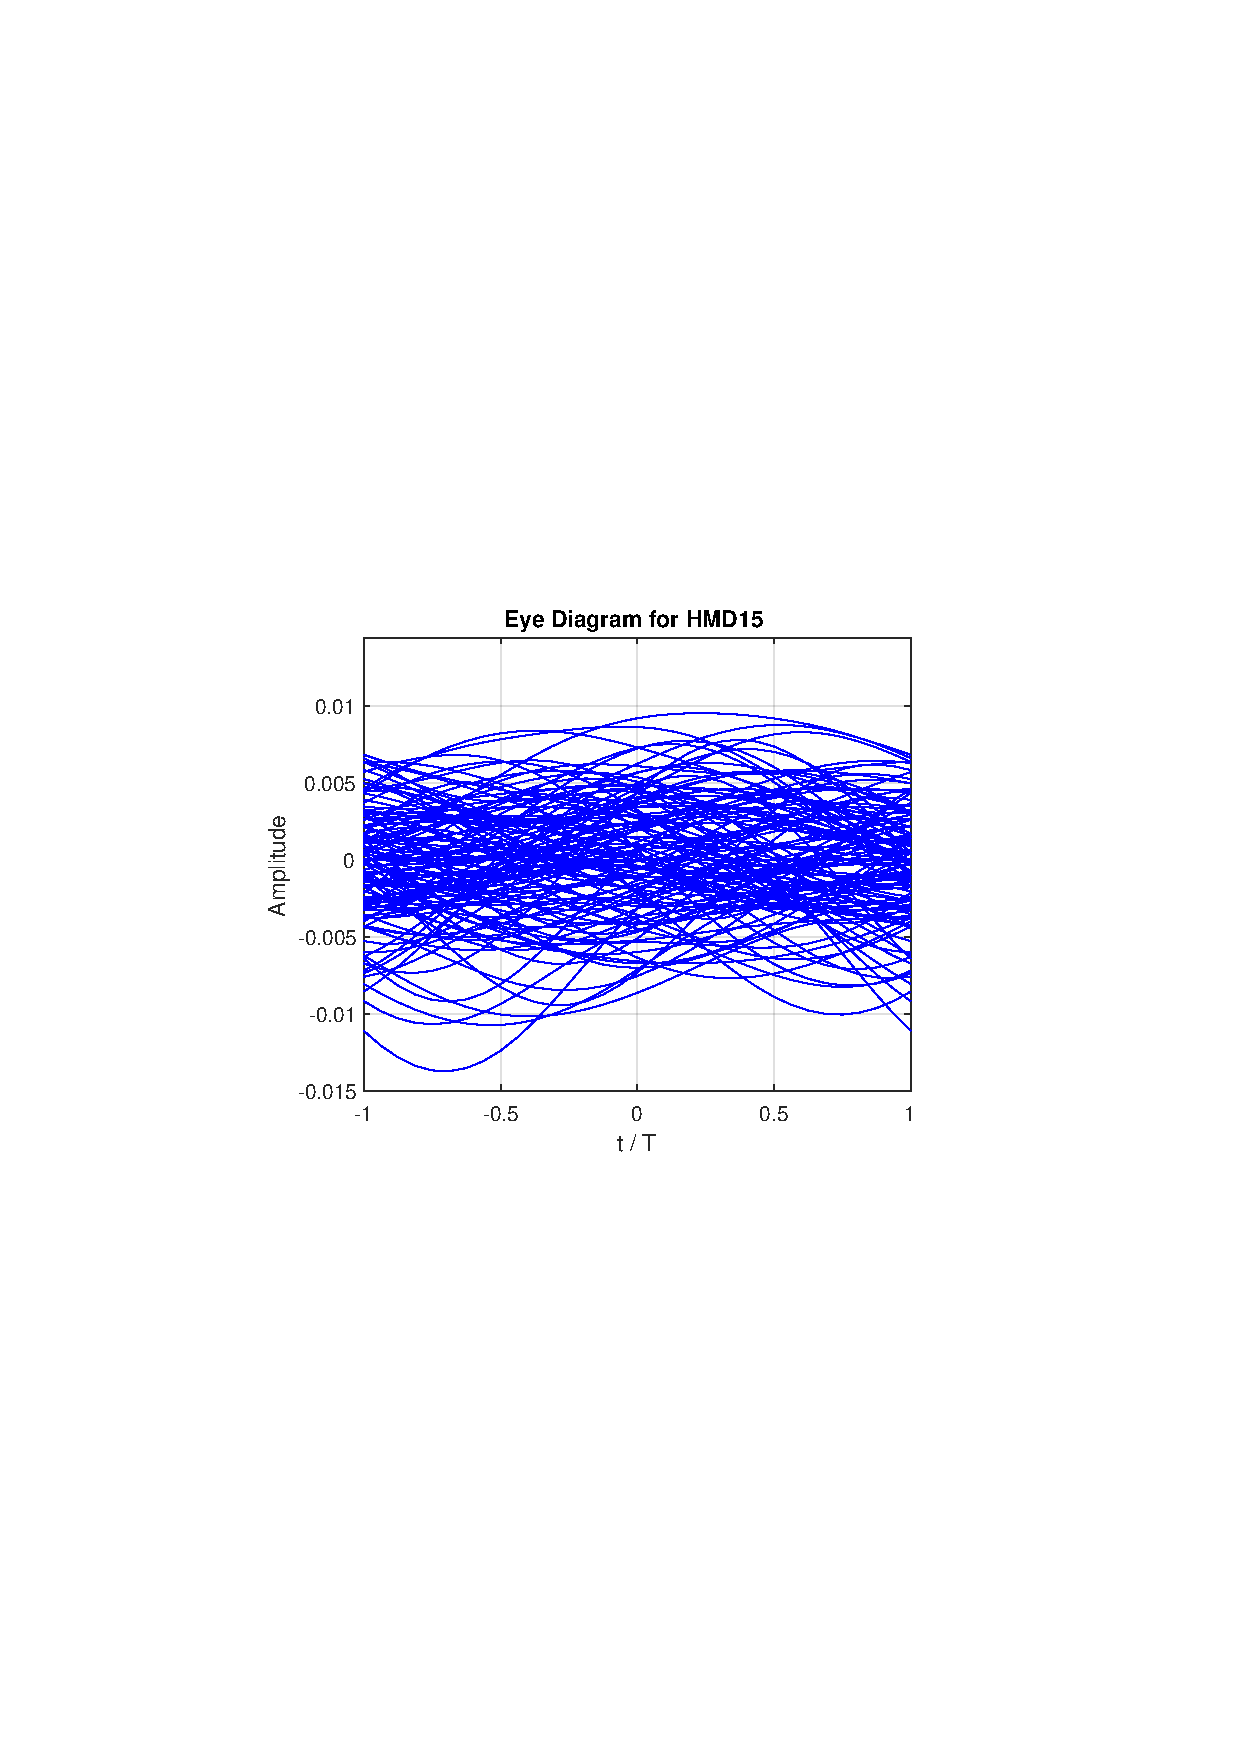
\includegraphics[clip, trim=5cm 10cm 5cm 10cm, width=\textwidth]{./sdf/m_qam_system/figures/HMD15_eye_diagram_140.pdf}
	\end{subfigure}
	\caption{Eye diagrams for the signals HMD14 (left) and HMD15 (right) for signalOutputPower\_dBm $=-140$. This corresponds to $\sqrt{\frac{E_b}{n_0}}=10^{-8}$.}
	\label{fig:eye_diagram_140}
\end{figure}

\begin{figure}
	\centering
	\begin{subfigure}{.5\textwidth}
		\centering
		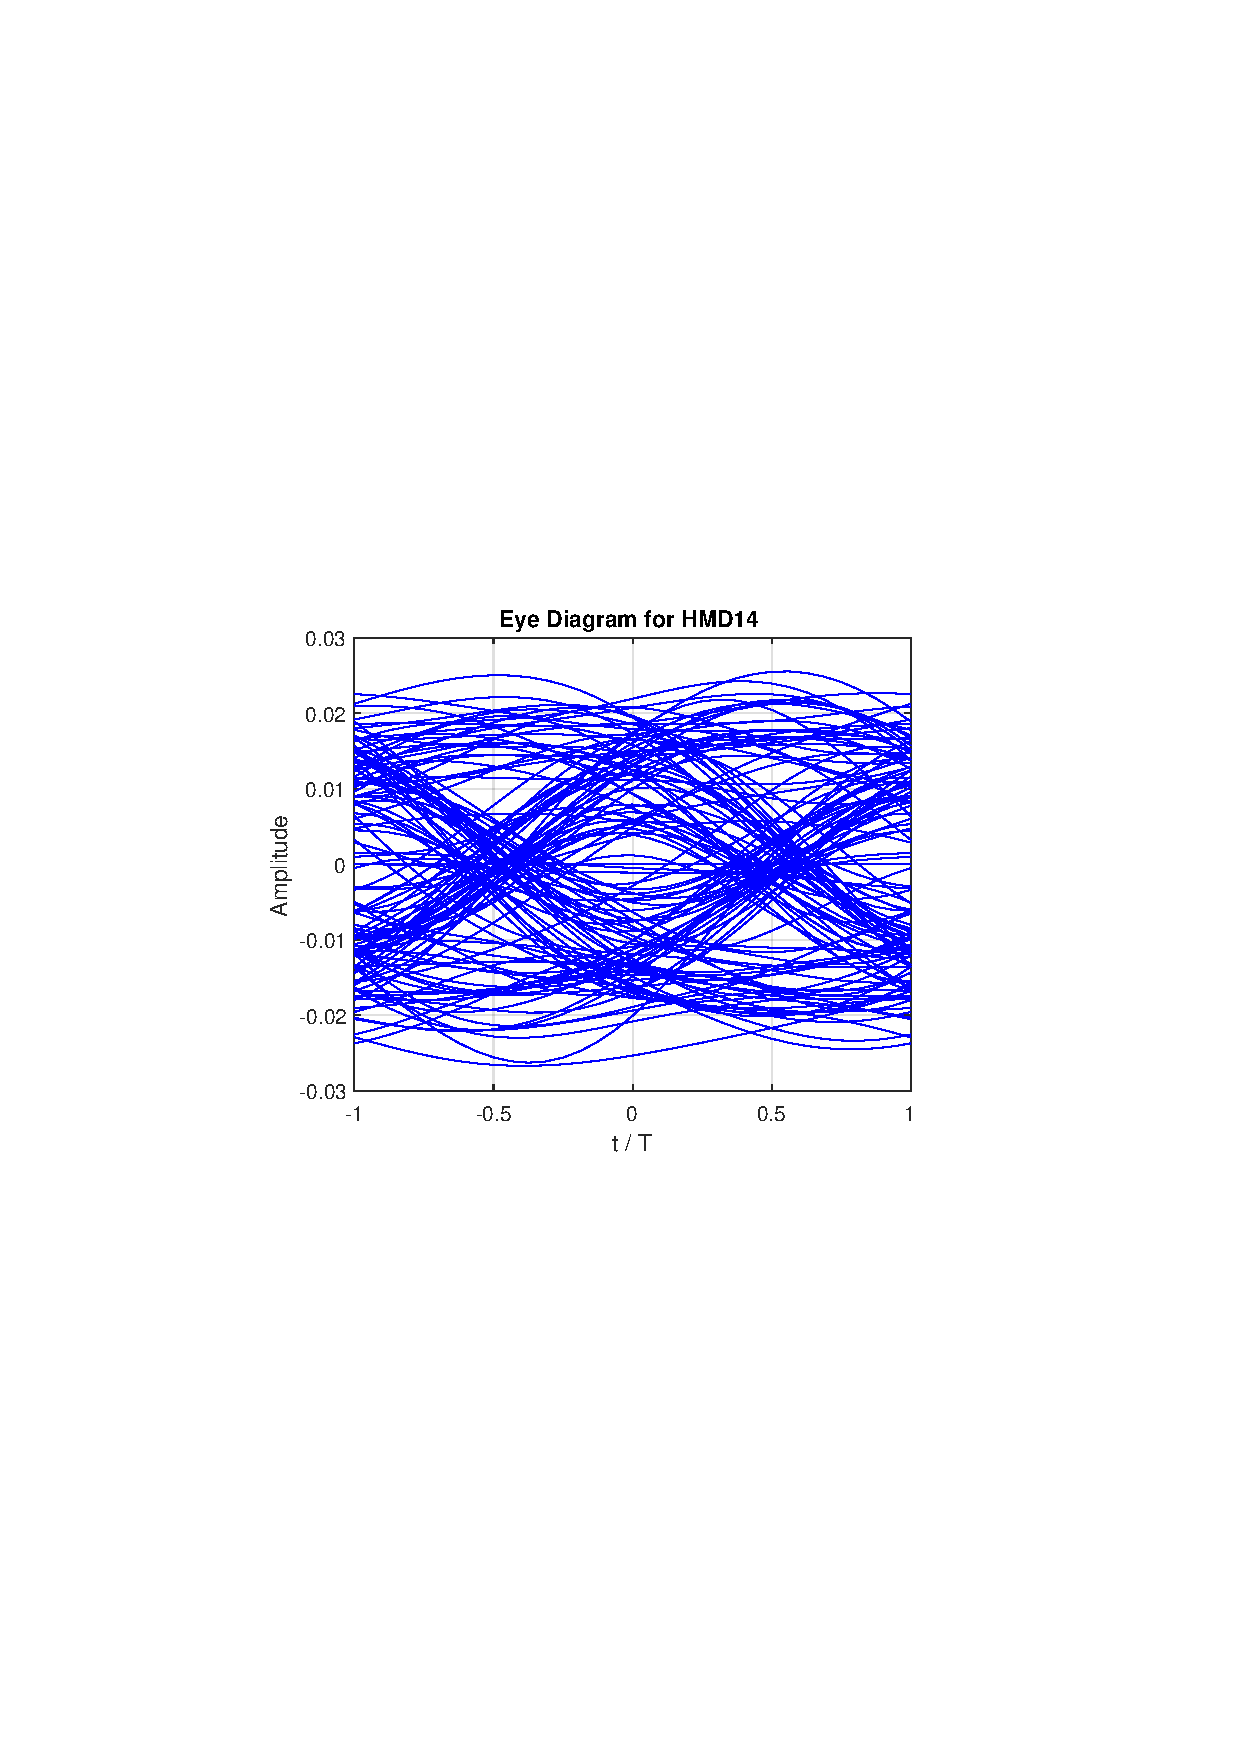
\includegraphics[clip, trim=5cm 10cm 5cm 10cm, width=\textwidth]{./sdf/m_qam_system/figures/HMD14_eye_diagram_60.pdf}
	\end{subfigure}%
	\begin{subfigure}{.5\textwidth}
		\centering
		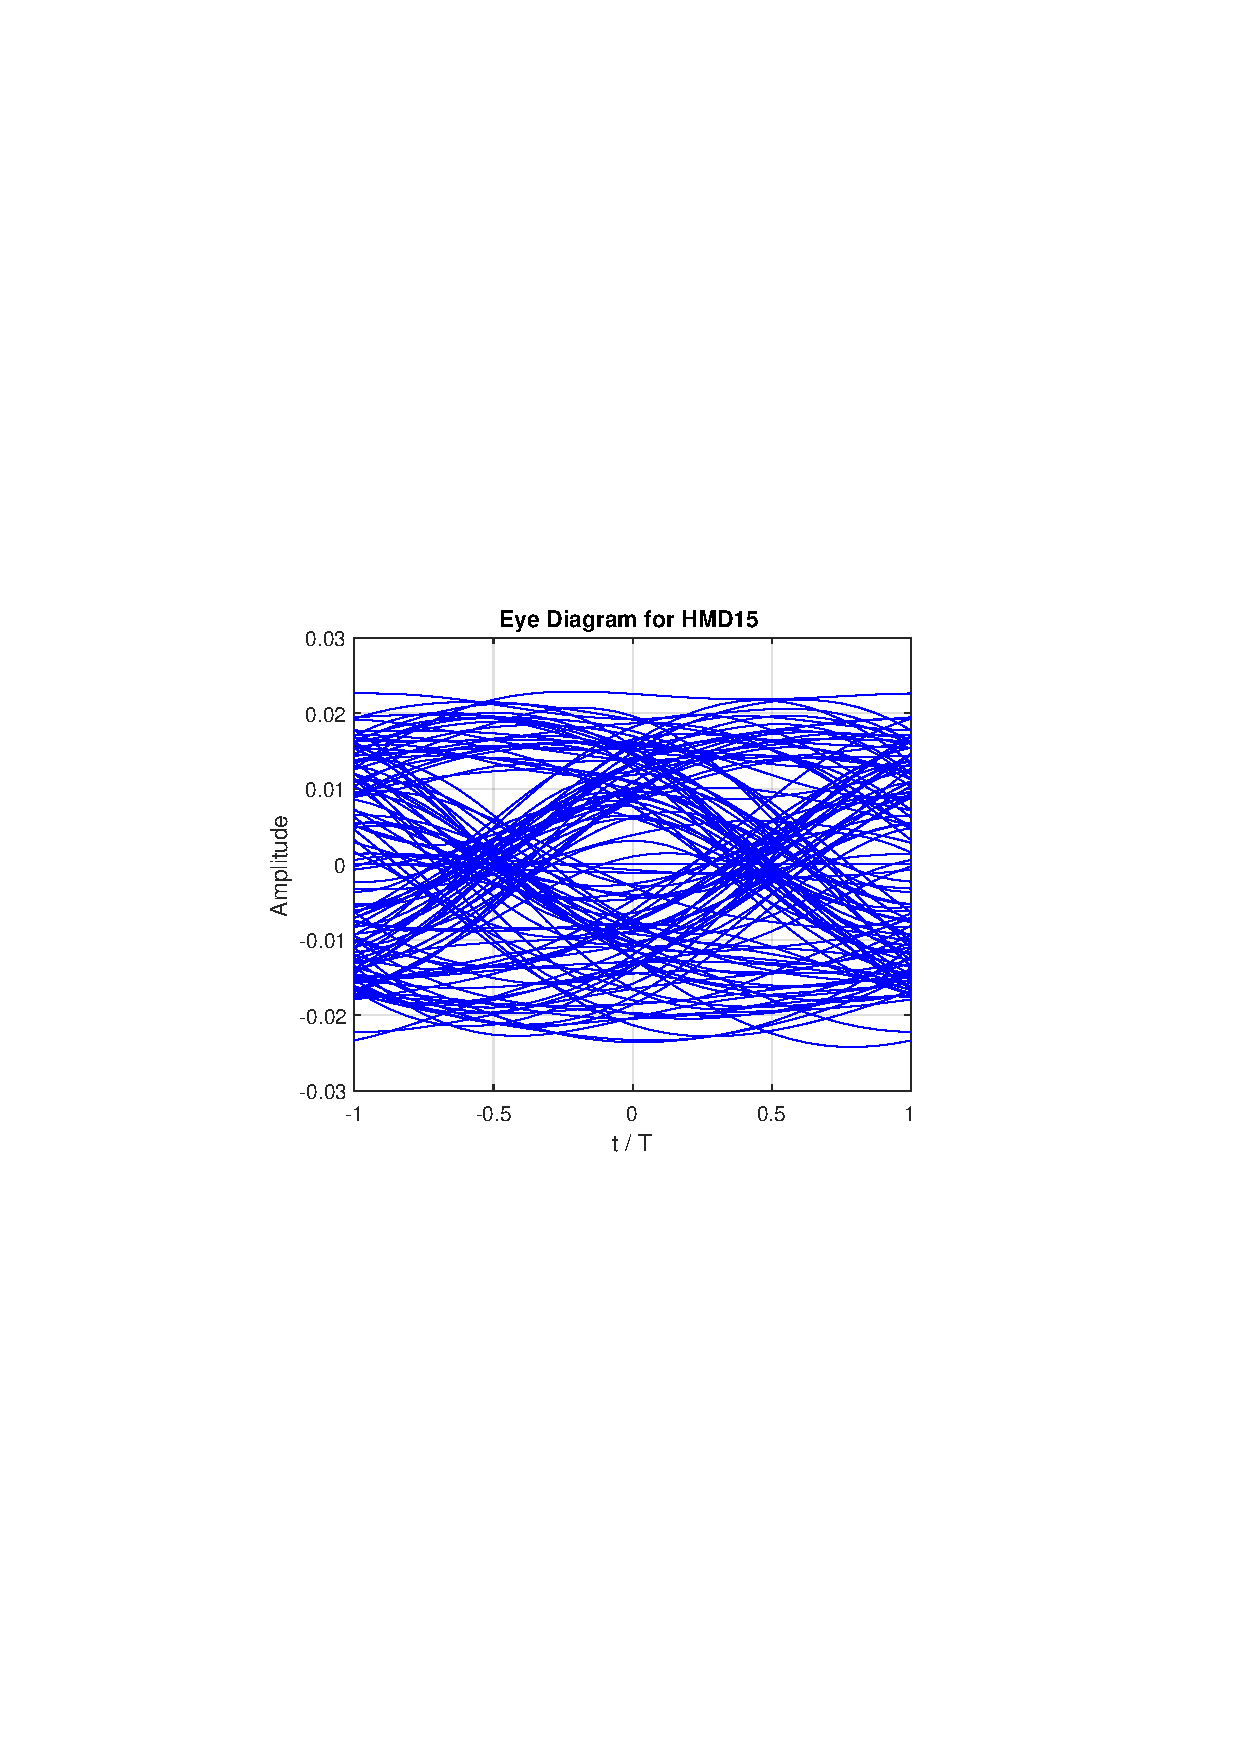
\includegraphics[clip, trim=5cm 10cm 5cm 10cm, width=\textwidth]{./sdf/m_qam_system/figures/HMD15_eye_diagram_60.pdf}
	\end{subfigure}
	\caption{Eye diagrams for the signals HMD14 (left) and HMD15 (right) for signalOutputPower\_dBm$=-60$. This corresponds to $\sqrt{\frac{E_b}{n_0}}=1$.}
	\label{fig:eye_diagram_60}
\end{figure}

